\documentclass[sigplan,preprint,10pt]{acmart}\settopmatter{printfolios=true,printccs=false,printacmref=false}
\settopmatter{printacmref=false}
\renewcommand\footnotetextcopyrightpermission[1]{}
\pagestyle{plain}

\usepackage{lineno,hyperref,xcolor}
\usepackage{flushend}
\usepackage{stmaryrd}
\usepackage{amssymb}
\usepackage{xypic}
\usepackage{semantic}
\usepackage{booktabs}
\usepackage{subcaption}
\usepackage{enumitem}
\usepackage{enumerate}
\setlist{leftmargin=6mm}

%\acmConference[PL'17]{ACM SIGPLAN Conference on Programming Languages}{January 01--03, 2017}{New York, NY, USA}
%\acmYear{2017}
%\acmISBN{} % \acmISBN{978-x-xxxx-xxxx-x/YY/MM}
%\acmDOI{} % \acmDOI{10.1145/nnnnnnn.nnnnnnn}
\startPage{1}
\setcopyright{none}
\bibliographystyle{ACM-Reference-Format}

\title{Wrattler: \textnormal{A platform for AI-assisted data science}}

\author{AIDA Team, The Alan Turing Institute}
%\affiliation{
%  \institution{The Alan Turing Institute}
%  \country{London, United Kingdom}
%}
%\email{tomas@tomasp.net}


\definecolor{cmtclr}{rgb}{0.0,0.6,0.0}
\definecolor{kvdclr}{rgb}{0.0,0.0,0.6}
\definecolor{numclr}{rgb}{0.0,0.4,0.0}
\definecolor{strclr}{rgb}{0.4,0.4,0.0}
\definecolor{rstrclr}{rgb}{0.5,0.1,0.0}
\definecolor{prepclr}{rgb}{0.6,0.0,0.2}
\newcommand{\vect}[1]{\langl #1 \rangl}
\newcommand{\langl}{\begin{picture}(4.5,7)
\put(1.1,2.5){\rotatebox{60}{\line(1,0){5.5}}}
\put(1.1,2.5){\rotatebox{300}{\line(1,0){5.5}}}
\end{picture}}
\newcommand{\rangl}{\begin{picture}(4.5,7)
\put(.9,2.5){\rotatebox{120}{\line(1,0){5.5}}}
\put(.9,2.5){\rotatebox{240}{\line(1,0){5.5}}}
\end{picture}}
\newcommand{\ball}[1]{\FPeval{\result}{clip(201+#1)}\textnormal{\ding{\result}}}
\newcommand{\lsep}{~\,|\,~}
\newcommand{\num}[1]{\textcolor{numclr}{#1}}
\newcommand{\str}[1]{\textnormal{\textcolor{strclr}{\sffamily "#1"}}}
\newcommand{\strf}[1]{\textnormal{\textcolor{strclr}{\sffamily #1}}}
\newcommand{\rstr}[1]{\textnormal{\textcolor{rstrclr}{\sffamily "#1"}}}
\newcommand{\ident}[1]{\textnormal{\sffamily #1}}
\newcommand{\qident}[1]{\textnormal{\sffamily \guillemotleft #1\guillemotright}}
\newcommand{\dom}{\ident{dom}}
\newcommand{\kvd}[1]{\textnormal{\textcolor{kvdclr}{\sffamily #1}}}

\newcommand{\bndclr}[1]{\textcolor{kvdclr}{#1}}
\newcommand{\bkndclr}[1]{\textcolor{prepclr}{#1}}
\newcommand{\blblclr}[1]{\textcolor{numclr}{#1}}
\newcommand{\bnd}[1]{\textnormal{\textcolor{kvdclr}{\sffamily #1}}}
\newcommand{\bknd}[1]{\textnormal{\textcolor{prepclr}{\sffamily #1}}}
\newcommand{\blbl}[1]{\textnormal{\textcolor{numclr}{\sffamily #1}}}


\begin{document}
\maketitle

\section{Introduction}
Data science is an iterative, exploratory process that requires a collaboration between a
computer system and a human. A computer can provide advice based on statistical analysis of the
data and discover hidden structures or corner cases, but only a human can decide what those mean
and decide how to handle them in scripts. Data science is often cited as an expensive
and time consuming task, especially due the costs of data cleaning and data wrangling.
We propose four fundamental reasons why
practical data science is expensive:

\paragraph{Big data is big,}
so the analyst doesn't understand it all.*
Even if a data set is small enough fits on one computer, it's still too large to fit in
an analyst's working memory.
But this means every analysis is huanted
by the spectre of lurking, potentially
unknown data quality  issues.
This also makes it more difficult to do data fusion, because there may be corner cases that make it more difficult to join two disparate data sources than expected.

\paragraph{The double Anna Karenina principle.}
Not only is every dirty data set  dirty in its own way, but \emph{pace} Tolstoy, every clean data set is clean in its own way as well.
"Data" is such an abstract concept that specific integrity conditions to characterize whether data is dirty, and potentially even the most appropriate formalism for integrity conditions,  differ dramatically across
the vast array of disparate use cases of data science,
ranging from relational data describing the customers of a country, time series data describing sensor data in an internet of things platform, and huge datasets of satellite imagery of the earth over a multi-year time scale.

\paragraph{Death by a thousand cuts.}
Often data transformation and processing steps are individually  very simple. But  there may need to be lots of them, and
because big data is big,
an analyst never knows if she has found them all.

\paragraph{Feedback cycles everywhere.} Data science is
not a pipeline but a connected mess of epicycles. This is because every step
in a data analysis actually teaches
the analyst more about the data and the problem, which might require rehtinking the earlier steps.
For example, there might be data quality issues that
are not uncovered until the analyst
investigates the output of a regression model.

\vspace{1em}
\noindent
To meet these challenges, we present Wrattler,
a new type of system for data science
that aims to transform the process
of data analysis.
Wrattler combines the interactive and literal programming paradigms
of notebook systems such as Jupyter
with new advances in AI systems for data wrangling and in provenance.
The main design principles are:

\paragraph{Interactive.} Interactivity
is necessary because ``big data is big''. The analyst learns about
the data set and the problem as she explores it.
Wrattler enables an efficient interaction by bringing computation closer to the human.
Wrattler notebooks run in the browser, cache partial results of computations and provide previews
of script results on-the-fly.

\paragraph{Reproducible.}
Data analyses must be reproducible
because of feedback cycles. As the
analyst learns more about the problem,
this may uncover data cleaning or preparation issues that require
redesigning and rerunning the analysis.
Wrattler separates the task of running scripts from the task of managing state.
This is handled by a data store, which tracks the provenance and semantics of data, supports
versioning and keeps the history, making the data analyses fully reproducible.

\paragraph{Polyglot.}
Modern data science naturally draws
on many competing languages and libraries, such as R and Scipy. As a side effect
of our interactive, reproducible design,
we obtain nearly for free the ability
to support polyglot data analyses.
Multiple languages can be used in a single notebook and share data via the data store.
Analysts can use R and Python, but also interactive languages for data exploration
that run in the browser and provide live previews.

\paragraph{Smart.}
AI can examine and find patterns
in big data where a human cannot,
again aiming at the problem that
big data is big.
AI can be used to direct the analyst's attention and to generalize  decisions about data transformation
to new data that that the analyst
hasn't seen.
Wrattler serves as a platform for AI assistants that use machine learning to provide suggestions
about data. Such AI assistants connect to the data store to infer types and meaning of data, provide
help with data cleaning and joining, but also help data exploration by finding typical and atypical
data points and automatically visualizing data.

\paragraph{Explainable.}
The hints provided by AI assistants are explainable. Rather than working as black boxes that
transform one dataset into another, AI assistants generate scripts in simple domain-specific
languages, that specify how the data should be transformed. Those scripts can be reviewed
and modified by a human.

\vspace{0.5em}
\noindent
In the rest of this document, we discuss limitations of current notebook systems and how Wrattler
resolves them (Section~\ref{sec:overview}). We discuss how the individual components of Wrattler
work together (Section~\ref{sec:wrattler}) and then focus on two of them in detail --
we look at how Wrattler can be extended with AI assistants (Section~\ref{sec:ai}) and
how semantic information about data is managed by the data store (Section~\ref{sec:datastore}).


\section{Wrattler and notebooks}
\label{sec:overview}

Notebook systems such as Jupyter have become a popular programming environment for data science, because
they support gradual data exploration and provide a convenient way of interleaving code with
comments and visualizations. However, notebooks suffer from a number of issues that hamper
reproducibility and limit the possible interaction model.

Notebooks can be used in a way that breaks reproducibility. The state is maintained by a \emph{kernel}
and running a code in a cell overwrites the current state. There is no record of how the current
state was obtained and no way to rollback to a previous state. The fact that the state is
maintained by the kernel means that it is hard to combine multiple programming languages and
other components such as AI assistants. Finally, notebooks provide a very limited interaction
model. To see the effect of a code change, an entire cell and all subsequent cells need to be
manually reevalutated.

The architecture of Wrattler allows us to address these issues, as well as to provide a platform
for building novel AI assistants and interactive programming. The architecture is illustrated
in Figure~\ref{fig:arch}. The components of Wrattler are:

\vspace{-0.25em}
\paragraph{Data store.} Imported external data, results of running scripts and of
applying AI assistants are stored in the data store. It stores versioned data frames with
metadata such as types, inferred semantics, data formats or provenance.

\vspace{-0.25em}
\paragraph{Language runtimes.} Scripts are evaluated by one or more language runtimes.
The runtimes read input data from and write results back to the data store.

\vspace{-0.25em}
\paragraph{AI assistants.} When invoked from the notebook, AI assistants read data
from data store and provide hints to the analyst. They help to write data cleaning
scripts or annotate data with additional metadata such as inferred types.

\vspace{-0.25em}
\paragraph{Notebook.} The notebook is displayed in a web browser and orchestrates
all other components. The browser builds a dependency graph between cells or individual
expressions in the cells. It calls language runtimes to evaluate code that has changed,
AI assistants to provide hints and reads data from the data store to display results.

\section{Wrattler components}
\label{sec:wrattler}

Wrattler consists of a user interface running in the web browser, which communicates with
a number of server-side components. In this section, we discuss the components in more 
detail, starting with the dependency graph that is maintained on the client-side, by the 
web browser. AI assistants are discussed later in Section~\ref{sec:ai}.

\subsection{Dependency graph}

When opening a notebook, Wrattler parses the source of the notebook (consisting of text cells and
code cells) and constructs a dependency graph, which serves as a runtime representation of the
notebook.

As an example, the graph in Figure~\ref{fig:deps} represents the notebook in Figure~\ref{fig:notebook}.
Top-level nodes (squares) represent individual notebook cells. Code (circles) is represented either as
a single node (Python, JavaScript) or as a sub-graph with node for each operation (cleaning DSL
understood by Wrattler). Any node of a cell can depend on a data frame (hexagons) exported by an
earlier cell. When code in a cell changes, Wrattler updates the dependency graph, keeping existing
nodes for entities that were unaffected by the change.

The dependency graph enables several features that are difficult for most notebook systems:
%
\begin{itemize}
\item[--] When code changes, Wrattler only needs to recompute a small part of the graph.
  This makes it possible to provide live previews, especially for simple data analytical DSLs.
\vspace{-0.85em}
\item[--] Refactoring can extract parts of the notebook that
  are needed to compute a specified output.
\vspace{0.25em}
\item[--] Refactoring can translate nodes of an analytical DSLs (generated by an AI assistant) into R or Python.
\vspace{0.25em}
\item[--] The graph can be used for other analyses and refactorings, such as provenance tracking
  or code cleanup.
\end{itemize}

\begin{figure}
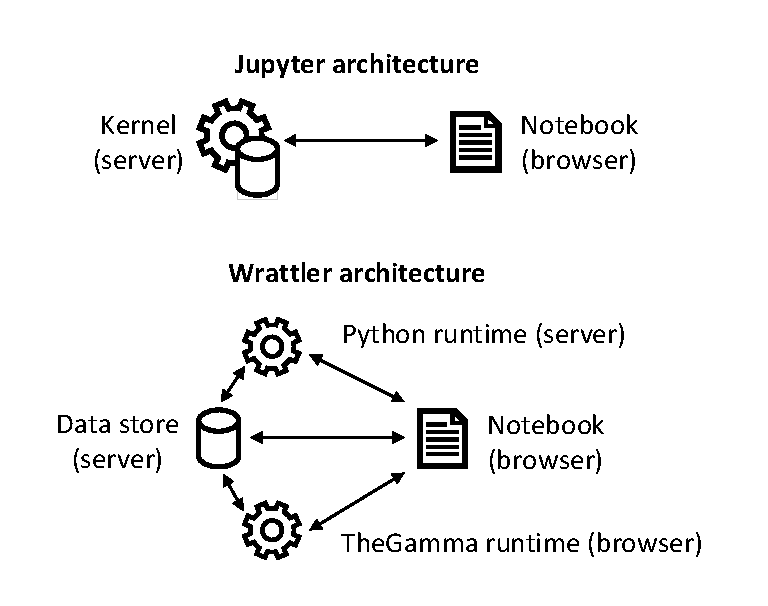
\includegraphics[scale=0.6]{diagram.pdf}
\caption{\small{In notebook systems such as Jupyter, state and execution is managed by a kernel. In
  Wrattler, those functions are separated and enriched with AI assistants.}}
\label{fig:arch}
\end{figure}


\subsection{Data store}
\label{sec:wrattler-ds}

The data store provides a way for persistently storing data and enables communication between
individual Wrattler components. Data store keeps external data files imported into Wrattler,
as well as computed data frames (and, potentially, other data structures). It is immutable
and keeps past versions of data to allow efficient state rollback. For persistency and versioning,
data store also serializes and stores multiple versions of the dependency graph.

The data store supports a mechanism for annotating data frames with additional semantic information, such as:
%
\begin{itemize}
\item[--] Columns can be annotated with (and stored as) primitive data type such as date or floating-point number.
\vspace{0.25em}
\item[--] Columns (or a combination) can be annotated with semantic annotation such as geo-location or address.
\vspace{-0.85em}
\item[--] Columns, rows and cells of the data frame can be annotated with other metadata such as provenance.
\end{itemize}

\noindent
The format of the annotations as well as other features of the data store are discussed in
more detail in Section~\ref{sec:datastore}.

\begin{figure}
\begin{equation*}
\begin{array}{l}
\textit{\small{In the first block, we retrieve data from a government web site.}}\\[-0.1em]
\textit{\small{We use Python to download the data and parse it as a CSV file.}}\\[0.3em]
\quad\ident{url}=\ident{open}(\str{http://data.gov.uk/\ldots/bb2014.csv})\\
\quad\ident{bbRaw}=\ident{csv.reader}(\ident{url})\\[0.2em]
\textit{\small{In the next block, we used an AI assistant to assist with cleaning}}\\[-0.1em]
\textit{\small{and created a script that marks \#!NULL values as missing:}}\\[0.3em]
\quad\kvd{let}~\ident{bbClean} = \ident{bbRaw}.\ident{missing}.\ident{as\_missing}(\str{\#!NULL})\\[0.3em]
\textit{\small{Finally, we use JavaScript to create a histogram of upload speeds:}}\\[0.3em]
\quad\ident{vega}.\ident{hsit}(\ident{bbClean}, \str{Upload speed})
\end{array}
\end{equation*}
\vspace{-0.5em}
\caption{\small{A small notebook consisting of three cells. The first Python cell exports
\ident{bbRaw}; the second Wrattler cell uses it and exports \ident{bbClean} and the
JavaScript cell visualizes \ident{bbClean}.}}
\label{fig:notebook}
\end{figure}

\subsection{Language runtimes}

Language runtimes are responsible for evaluating code and assisting with code analysis during
the construction of dependency graph. They can run as server-side components (e.g.~for R and Python)
or as client-side components (in case of JavaScript).
Unlike Jupyter kernels, a language runtime is stateless. It reads data from and writes data to
the data store (using a cache for efficiency).

\section{AI assistants}
\label{sec:ai}

{
An AI assistant is a component
of the system that
guides data analysts through a single data collection, integration, preparation,
analytics, or reporting task.
For example, an assistant might
specialize in identifying suspicious
values, such as "-1" in a column labelled
"heart rate", which might indicate
that certain data was not collected.
Assistants are interactive, in that
they propose a transformation
of the data to the analyst, based on combinations
of statistical and symbolic AI analysis,
and then refine the transformation
based on feedback from the analyst.
Typically analysts will interact with many separate assistants over
the course of an analysis, each of which specialize in a single kind of task.

\subsection{Architecture of AI assistants}

There are two important design aspects of AI assistants, which may seem
contradictory.
 First, they must be interactive, following
 the first principle behind Wrattler, but
 following the second,
 they must also be reproducible.
We square this circle by using the notebook
system as a reproducible interlingua.
The output of an AI assistant is always code, rather
than being a black-box that transforms data,
and it is this code that is agreed between the AI and the analyst during the interaction.
Thus the interaction is viewed as a ``design phase''
that is not reproduced on new data.

More specifically, an AI assistant defines a domain specific language (DSL) for the task at hand. When invoked from
a notebook, it guides the user in creating a script in the DSL. Running the script performs
the required operation (such as data cleaning). The assistant defines the semantics
of those operations and, when the script is executed, stores the result into a data
store. This new data frame can contain new data or additional information (such as their
inferred types).
The interaction is illustrated in Figure~\ref{fig:arch}. An AI assistant reads data from the data
store and returns suggestions to the notebook, which the user can review and accept.

Assistants are therefore based on two different ideas:

\begin{figure}
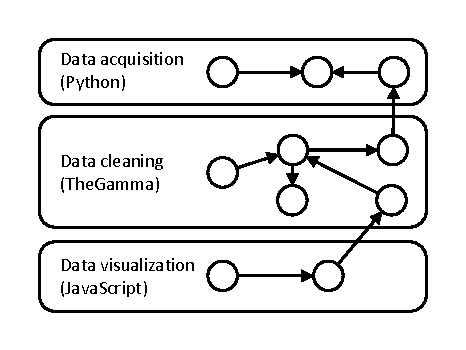
\includegraphics[scale=1,trim=0.5cm 0.5cm 0.5cm 0.5cm]{graph.pdf}

\caption{\small{Dependency graph for the notebook in Figure~\ref{fig:notebook}.
Data acquisition is represented as a single Python cell. Data cleaning is understood
by Wrattler and is the graph has a node for each call and constant. Hexagons represent
data frames shared by cell and stored in the data store.}}
\label{fig:deps}
\vspace{-0.5em}
\end{figure}

\paragraph{Domain specific languages.}

Wrattler includes a scripting language with simple syntax that is used
by individual AI assistants to define domain specific languages. The
syntax is shared across multiple AI assistants, but the operations are
provided by individual assistants.

For example, an AI assistant based on datadiff
guides the user in writing scripts that transform a malformed data frame into a correct format
specified by a correct data frame. The resulting script might look as follows:
%
\begin{equation*}
\begin{array}{l}
\ident{datadiff(broadband2014, broadband2015)}\\
\quad.\ident{drop\_column}(\str{WT\_national})\\
\quad.\ident{drop\_column}(\str{WT\_ISP})\\
\quad.\ident{recode\_column}(\str{URBAN}, [\num{1}, \num{2}], [\str{Urban},\str{Rural}])
\end{array}
\end{equation*}
%
The script specifies that two columns should be dropped from the badly structured data frame and
one column needs to be recoded (turning $\num{1}$ and $\num{2}$ into strings
\strf{Urban} and \strf{Rural}).

The code produced by an AI assistant can be used in two ways. First, the analyst writes the code
interactively during an interaction with the AI assistant. During this phase, Wrattler
keeps a fine-grained representation of the code in the dependency graph (second cell in
Figure~\ref{fig:deps}), which allows Wrattler to provide live previews of the result, giving the
user an immediate feedback.

At a later stage, when the code is used in production, the code can be translated to a language
like R or Python. This translation uses the fine-grained representation of the code in the
dependency graph and maps individual nodes to corresponding Python or R functions.

\paragraph{Interactivity.}

Assistants should usually contain user interaction in their design, and adapt rapidly to feedback
from the analyst. For example, a data cleaning assistant would probably want to ask the user to
confirm potential changes, and if the user says no, to reconfigure the cleaning module
significantly so that the user does not need to keep rejecting similar changes.

In the above example, the interaction is provided through the ``.'' operator of the scripting
language. When the analyst types the first line to invoke the AI assistant and types ``.''
the datadiff assistant offers the most likely patches and the user can choose which ones
to accept. 

Scripts consisting of a chain of simple method calls are readable, allowing the data analyst to look at them
and verify that the transformations accomplish the intended task (such verification further
benefits from live previews that Wrattler provides when the analyst navigates through the
individual transformations).

At the same time, AI assistants can be used in a fully automatic ``batch mode'' by analysts
who already know what they want to achieve and know that the assistant produces the result they
require. In this case, Wrattler will simply automatically accept the default recommendations made
by an AI assistant. This allows packaging the assistant as an equivalent of scikit-learn for
data preparation.

\vspace{1em}
\noindent
The Wrattler architecture supports the development of AI assistants in a number of ways. First, AI
assistants have access to the data store and can use it to provide guidance about both data and
code. Second, Wrattler includes an extensible framework for defining domain-specific languages
(DSLs) that can describe, for example, data extraction, cleaning, transformation or visualization.

The data store provides AI assistants with
two sources of information that they can exploit
to determine what guidance to provide the analyst:
%
\begin{itemize}
\item[--] AI assistants can access all data stored in the data
store. This includes imported external data files, such as raw text or raw HTML content from which
the analyst wants to extract data, as well as structured data frames imported from CSV files or
produced as a result of previous computations. Moreover, an AI assistant can also access multiple
versions of a file.

\item[--] AI assistants can access the dependency graph created for a
notebook. This allows them to access the transformation history, which is the code
that has already been run during the analysis. This gives assistants information about the
context such as transformations that have already been performed.
\end{itemize}

\medskip \noindent
The assistants should be self-contained in the sense that they interact with each other
only through the
data store. This restriction is necessary in order
for provenance tracking and reproducibility.



\subsection{The Assistant Landscape}
{

AI assistants can be imagined for every step of the data analytics process.
To give an idea of the breadth of this framework,
we present a broad list of the data analytics tasks which have potential for assistant automation.
This is an intentionally broad list, more so than
could be fully explored in even a large research project, but gives a sense of the breadth of
potential use cases of our framework.

\paragraph{Data collection.} Assistants can search the data store, as well as external repositories
to recommend data sets that are relevant to the task at hand and offer to import these. For example,
when analysing data about different countries,
the assistant could suggest joining in public
demographic information from DBPedia.

\paragraph{Data integration} is a problem as common
as it is difficult. We envisage assistants
that combine logical and statistical reasoning to assist
with data  integration. A simple but useful
example of a tool in this space is to
 identify pairs of variables across multiple data
sources that are likely to be daily temperatures.
More sophisticated examples could include and extend the
most cutting edge techniques in the data fusion and
semantic technologies literatures.

\paragraph{Schema inference.} A sad fact of data
science is that data sets are often not as well documented
as we might like, even to the minimal level of
documentation of the types of each column.
There is an interesting opportunity to
develop machine learning methods that inferring types of variables from their values, e.g.,
by noticing that integer values between 0 and 30 in
the United Kingdom might describe an outdoor temperature, especially if other weather-related
variables are detected in the data set.

\paragraph{Data parsing.}
A common task in data analysis is to convert
data that is ``almost'' in structured form,
such as HTML tables, into a relational table.
Assistants in this space include
tools specifying a scraper for web pages, related
to wrapper induction \cite{Kushmerick1997WrapperIF},
for inferring format of CSV files (while simple
conceptually, they have no standard format), and
for extracting tables from html and pdf files
\cite{pinto03table}.

\paragraph{Data cleaning} is a well studied
problem in the databases and data mining literature
\cite{abedjan2016detecting,ilyas2015},
but there are still a huge number of issues that have been unexplored.
For example, we envisage assistants for:
identifying values that seem to be out of range, e.g. missing value indicators;
identifying possible inconsistent coding of strings,
such as different representations of acrynoms;
identifying rows that seem "jointly" unusual, i.e., that seem not to conform to statistical dependencies among the columns; and
identifying distinct records that may refer to the same entity (record linkage).

\paragraph{Data monitoring.} Once an analysis
is completed, it may result in a machine learning
model which will then be deployed on a data stream.
Once a classifier is deployed, it must be monitored
to detect shifts in its input distribution,
such as change points, covariate shift, and
concept drift. This includes the problem
of suggesting when/how often new data points should be labelled for monitoring.
Even for data analyses that do not involve
deploying a ``production model'', there is
often a need to run an analysis periodically on updated data, such as
re-running last quarter's analysis on this quarter's data.
In such cases, we might believe that the two data
sets come from approximately the same distribution
and format, so we can exploit
divergences from this assumption to indicate
potential issues with data quality.
As part of the Wrattler effort, we have
introduced the \emph{data diff} problem \cite{datadiff},
which aims to improve the process of data wrangling by
returning a report of the differences between two data sets.

\paragraph{Exploratory visualization} to summarize
data sets, both the target data of the analysis,
and the results of transformations that the analyst
creates. Potential assistants here include ones
to summarize most representative rows of a data table,
and automatically choosing appropriate interactive
visualizations, such as scatterplots and bar charts,
with styling decisions such as axes automatically
chosen to be most informative.

\paragraph{Performing analytics.}
An increasing amount of attention is being
given to the AutoML challenge \cite{guyon_review_2016}, which focuses
on automatically choosing a classification
methods, feature representations and hyperparameters
for a given classification task, without the need for human intervention.

\paragraph{Debugging and interpreting predictive analytics.}
Every time a new machine learning model is trained, the first question
an analyst has is often why its accuracy is not better. But debugging
predictive analytics is notoriously difficult, and the remedies
indirect and expensive, e.g., labelling more data, adding more
features, using a more complex model. Debugging and improving models
is a rich area for potential assistants.  There is potentially low
hanging fruit available in how to aid the tasks of error analysis,
exploring the predictions of the model on validation data. Some early
work in this direction is \cite{saleema}.  There is a rich and growing
literature on interpreting and explaining the predictions of a model
\cite{lipton:mythos,doshi-velez17,ribiero2016lime,darksight}.  Two
potential directions from are debugging by using "training set
blame": Given an error in the validation data, what examples from the
training set caused me to make that error? This might build on the
work of \cite{percy}.  Another potential avenue is explaining
differences between predictions: why was instance 42 treated
differently than instance 24601, even though they appear highly
similar to a human?  }

%%cs possibly we don't need to go into detail
%% in this version of the report? Or we might
%% decide to add this back.
\begin{comment}
\subsection{Possible AI assistants}

Designing an AI assistant requires an intriguing
combination of data science, AI, and user interaction
thinking.
As an example of the types of design considerations
that arise, we go into more detail about the
design issues that arise when considering
three examples of the broader list of agents
in the previous section.

{\color{blue}

\paragraph{Data Parsing.}

Simple scraper assistant: Simple information extraction wizard. Create a data table based
on HTML pages that have been automatically generated, like product review pages,
for which a simple pattern on the HTML tree will be sufficient to extract the desired information.
This is called wrapper induction in the information extraction literature.

* *Input*: Web page that contains information in unstructured form, such as a list of search resuts or an HTML list.

* *Output*: A data frame (i.e. a relational table) that contains the information that has
been extracted from the web page.

* *User interaction*: User needs to initially highlight and specify which items to be scraped.
Need to summarize the results of the scraping and highlight cases
which might require correction from the user. Update scraper accordingly.

* *Potential method*: A wrapper is a path through the HTML DOM. Use a language (like XPath) for navigating through the DOM. Search for the shortest path that retrieves
the labels provided by the user.

* *Research issues*: Not clear, given the large amount of related work in this area.
We would need to read around carefully before we can identify opportunities.
Possible opportunities include:
    (a) Using a language like [Scrapy](https://scrapy.org/) to induce the wrappers;
    (b) Using a language model over the scraped values to fine-tune the wrapper (e.g. if a wrapper returns both dates and cities, it's probably wrong), or
	(c) using a probabilistic model over the program representation of the wrapper to focus attention in the search
for good wrappers. Perhaps there are enough scrapers on line (e.g. Github projects that use scrapy) that you can get a training set for this.
* *Related work*: Gulwani's work on data wrangling, lots of work on wrapper induction.
There is a lot of work on this. Scrapy is a popular open source framework that several
of my BSc/MSc students have found useful.

\paragraph{Data cleaning.}
*Inconsistent string assistant*: Identify potential typos in string data. The idea is to look for strings that do not occur commonly in the data set, but are very close in edit distance
to strings that do occur commonly.

* *Input*: A column of a data table whose values are strings, like addresses, cities, states/provinces, occupations, and so on.

* *Output*: A list of suggestions for strings that should be renamed: e.g. `[ ("Stocland", "Scotland"), ("Untied Kringdom", "United Kingdom") ]`

* *Potential method*: Simplest cut: Define a threshold $\delta$ on Levenshtein distance,
and $0 < \alpha < 1$ on the number of occurrences. Return the set of all strings $y$ that
occur less than $\alpha N$ times in the data set but where there is a corrected string $x$ which is less than $\delta$ in string edit distance from $y$.
More ambitious: Noisy channel model for correction.
Learn a probability distribution $p(x)$ over the strings in the column,
and  define an error model $p(x'|x)$. Then search for ways to transform the  dirty column $x'$  to a clean version $x$ in such a way to maximize $p(x|x')$.
This formulation deserves some more thought,
though, before we try to implement it.

* *Research questions*: Need to connect this to existing concepts in the databases and
data mining literature, such as U-repair.

* *User Interaction*: The user should be able to reject suggestions in the output list,
and this should rapidly update the models used in such a way that similar suggestions
to the bad ones are also removed from the list. A noisy channel model would be nice
for this, not sure about the edit distance one.

\paragraph{Exploratory visualization.}

*Data table summarization assistant*: Displays a short subtable of the most "representative"
columns of a given data frame. The number of rows in the summary should be small enough
to fit on a given screen. Essentially an alternative to the `head()` function in pandas/R.

*Input*:  A data frame, along with type information (continuous/categorical) for each of the columns. Desired number $k$ of rows in output.

*Output*: A list of $k$ indices of rows in the dataframe

*Potential method*:  Simplest possible implementation:
Run $k$-medoids and return the medoid values.

*Research questions:* First, are there research questions here, or is this so simple
that it  is part of the infrastructure?  If $k$-medoids is so simple for this,
why doesn't everyone also do it? How to evaluate whether the summary is good?
Maybe there are examples of data sets where medoids is not good.
For example, in the Karpathy ICML example, medoids would not make sense,
listing the institutions that have the most papers is most informative, because
it's a "long tail" type of column. How do you tell "long tail" data from "just show
the clusters" type data? Perhaps a model-based framework could distinguish?
Maybe you want to summarize the ways in which two data sets differ?
Is the best summary the cluster centroids or the "top k" along some value?
* *User interaction:* I'm not sure what interactions are enecessary.
Users could ask for more rows, mark two items as similar, or mark an item as uninteresting.
Or perhaps better would be to allow drill down, i.e., to make it easy to explore
the clusters represented by each example.
}
\end{comment}

\section{Data store}
\label{sec:datastore}

The data store links together individual components of Wrattler. It stores the raw input
data for data analysis such as downloaded web pages, raw data frames and also data frames
produced as the result of running a script or invoking an AI assistant. In addition to data,
the data store also stores multiple versions of the dependency graph created by Wrattler.

In the initial version of Wrattler, we restrict the data storage to raw input files and
data frames, however we note that it would be desirable to include other data structures
such graph or network data.

In this section, we focus on the initial functionality that is
required from the data store.  We focus on the public interface
exposed by the data store, but we do not discuss the technology used
for data storage -- this can be decided during the development.

Data frames stored in the data store can be annotated with
metadata. Such metadata can communicate information between multiple
AI assistants. For example, first AI assistant can infer that a pair
of columns represent GPS lat/lon coordinates and produce a data frame
with annotations specifying this information. A second AI assistant
can then use this information and automatically provide a data
visualization in the form of map. In the rest of this section, we
discuss the structure of those annotations.

\subsection{Semantic annotations}
As noted in Section~\ref{sec:wrattler-ds}, annotations can be attached to individual cells,
entire columns and rows, but also combinations of multiple columns or rows. As an example,
consider the following small table obtained from a government web site that records data 
on broadband speed (and illustrates a number of real-world problems):

\vspace{1em}
\begin{tabular}{llc}
\toprule
\textbf{ISP}\qquad\qquad\qquad & \textbf{Postcode}\qquad\qquad & \textbf{Download} \\
\midrule
Virgin & CB43BE & 46.34 \\
BT & CB43PT & N/A \\
Virgin & NW53HL & 41.2 \\
BT & London & 16.4 \\
\bottomrule
\end{tabular}
\vspace{1em}

\noindent
As a first step, the data analyst might use the probabilistic type inference (ptype) assistant
in order to infer the types of data in the data set. The assistant needs to be able to annotate
the table with the following information:
%
\begin{itemize}
\item[--] With high certainty, the ISP column is a categorical column with values Virgin and BT;
  with lower certainty, it could also be a string.
\item[--] The column Postcode is most likely a postcode; with lower probability it is a city name
  and with similarly low probability, it is a plain string.
\item[--] The column Download is most likely a number or a missing value represented as N/A.  
\item[--] The N/A cell is annotated as being most likely a missing value, or less likely a plain 
  string. Other cells of the Download column are annotated as most likely being decimal numbers.
\item[--] The cells of the Postcode column are annotated similarly. The first three are most
  likely postcodes, while the last one is most likely a city name, but all also have a non-zero
  probability of being an arbitrary string.
\end{itemize}

\noindent
Assuming the data frame is extracted from a government web page, each row of the data set
could further be annotated with the URL of the data source. This makes it possible to track
provenance at a fine-grained level. If we then append two such data frames, we will know
which row comes from which government data set.

It is worth noting that the data store does not need to fully understand the semantics of such 
annotations. The probabilistic type inference assistant simply adds them and another assistant
can then clean the data and, for example, drop values that do not conform to the most 
probable type. We return to this topic in Section~\ref{sec:datastore-schema}, after discussing
the format of such annotations.

\subsection{Annotation format}
The format of annotations needs to be light-weight so that it can be easily consumed and produced
by AI assistants created in a variety of different programming languages. For this reason, it is
desirable to use a standard file format such as JSON or XML. Furthermore, the format needs to 
be extensible -- although Wrattler should provide a schema for basic annotations, new AI assistants
should be able to freely define and use new kinds of annotations.

An annotation format that satisfies the above constraints can take inspiration from the 
Schema.org project (\url{http://schema.org}), which provides a way of annotating web content
with semantic information. The focus of Schema.org is on higher-level entities (such as 
a person, an event or a place), rather than lower-level information, but the format itself could
be reused by Wrattler.

\begin{figure}
\begin{equation*}
\begin{array}{l}
\{~~\; \str{@context}: \str{http://schema.org},\\
\quad  \str{@type}: \str{Place},\\
\quad  \str{name}: \str{The Black Lodge},\\
\quad  \str{address}: \{\\
\qquad    \str{@type}: \str{PostalAddress},\\
\qquad    \str{addressLocality}: \str{London},\qquad\qquad\qquad\qquad\qquad~\\
\qquad    \str{postalCode}: \str{NW53HL} ~\}~\}\\
\end{array}
\end{equation*}
\caption{\small{Example of a Schema.org annotation using a JSON encoding (it is worth noting 
that Schema.org also supports RDF).}}
\label{fig:schema}
\vspace{-1em}
\end{figure}

As an example, Figure~\ref{fig:schema} shows a Schema.org description of a place.
The \str{@context} attribute defines a namespace of a schema that defines the available
entities. The default namespace, used here, includes two entities that we use in this 
example, namely Place and PostalAddress.

The namespace mechanism provides a convenient way of extending annotations -- Wrattler can
define a core schema for common information that it needs, but new AI assistants can 
extend it via custom namespaces.

The Schema.org format also makes it easy to attach additional information to an existing
value. In the example above, the original value might have been ``The Black Lodge'', but 
an AI assistant -- possibly using entity linkage -- inferred and extended it with postal address.

\subsection{Schemas for data science}
\label{sec:datastore-schema}

Just like the default namespace of Schema.org defines common types of entities, Wrattler
should define basic schema for the most common annotations. This includes two kinds of annotations.
First, there are primitive type annotations that are understood by the data store. Second,
there are frequent semantic annotations that are generally useful. 

\paragraph{Schemas for primitive types.} The data store will store primitive values in the
data frame in a suitable native format such as floating-point number, Boolean, string or 
ISO 8601 date. However, this representation should remain internal and data store should be
able to consume and expose data in formats required by the client (this is further discussed
in Section~\ref{sec:datastore-negotiation}). This will be done through primitive type annotations.
The data store will understand those and will be able to convert between them automatically.
The primitive type annotations include:
%
\begin{itemize}
\item[--] \textbf{Numerical formats}. The data store will be able to convert between a number of common numerical
  formats such as integers, floats and unbounded size integers. In addition, values can also be
  formatted differently. Examples include the scientific notation (1.34e10) or variations in 
  decimal separators used in different cultures.
  
\item[--] \textbf{Dates}. The data store will be able to recognise and convert between a number of
  standard date formats (such as ISO 8601 format, dates in US and non-US formats).

\item[--] \textbf{Missing values}. The data store will record missing values internally and will be
  able to return them in a variety of formats, depending on the client request (NaN, special 
  strings such as empty or \#!NULL, etc).
   
\item[--] \textbf{Geo coordinates}. The list of primitive types might also include geographical
  coordinates, in which case the data store will recognize basic formats such as GPS coordinates  and Northings and Eastings.  

\end{itemize}

\noindent
The above primitive types need to be understood by the data store, in order to enable easy
communication between clients written in a variety of programming environments that use different
primitive types. The key idea is that each client will only need to handle, for example, one format 
for dates. The data store will be able to communicate using this format, even when the value was
written in another format by another client.

In addition, Wrattler should define a set of annotations that can be used by a wide range of
standard data sets. It is useful to provide a basic schema for such common annotations as this
will enable a range of AI assistants and other tools to exchange information without first having
to define a common custom schema. Those should include annotations for places (addresses, 
countries, cities, postcodes), physical units (meters, kilograms, etc.), contact information
(e-mails, phone numbers) and similar. We will investigate whether Schema.org or other existing
standards developed by the semantic web community already cover those areas.

\subsection{Content negotiation}
\label{sec:datastore-negotiation}

As noted earlier, the data store will understand a range of primitive data types and will be 
able to convert between them. This will be done using a content negotiation protocol,
similar to the Accept/Content-Type header pair in the HTTP protocol. Rather than using 
content type as in HTTP, the negotiation will be based on the schema. For example, a client may
specify that it accepts data with a certain namespace or that it recognizes a specified list of
types.

For primitive types that the data store understands, it will convert data according to the
request made by the client. For example, a date can be automatically converted between 
mm/dd and dd/mm formats. For additional semantic annotations that the data store does not
understand, it will simply drop the extra information not required by the client.

This makes it possible to exchange data efficiently. For example, a data frame where each cell
is annotated with a probabilistically inferred type will be significantly larger than a data
frame containing just raw numbers. The content negotiation protocol allows the client to 
request a data frame with just raw numbers, significantly reducing the size.

\bibliographystyle{plain}
\bibliography{paper}
\end{document}
